%%%%%%%%%%%%%%%%%%%%%%%%%%%%%%%%%%%%%%%%%%%%%%%%%%%%%%%%%%%%%%%%%%%%%%%%%%%%%%%%
%% Document Preamble
%%%%%%%%%%%%%%%%%%%%%%%%%%%%%%%%%%%%%%%%%%%%%%%%%%%%%%%%%%%%%%%%%%%%%%%%%%%%%%%%
\documentclass[a4paper,10pt]{report}

%% \usepackage[margin=0.5in,nomarginpar]{geometry}

%% Base Folder for Inputs
\makeatletter
\def\input@path{{../tex/}}
\makeatother

%% Import Packages
\usepackage{fvextra}
\usepackage{csquotes}
\usepackage{xcolor}
\usepackage{minted}
\usepackage{amsfonts}
\usepackage{amsmath}
\usepackage{enumitem}
\usepackage{graphicx}

%% Literate Haskell Macros

%%% include common formatting
\input{lhsfmt.tex}
%%% for ignoring some code
\long\def\ignore#1{}
%%% for creating a paragraph
\newcommand{\lhsparagraph}[1]{\paragraph{#1}\mbox{}\\}

%% Document Meta Data

\title{Denotational Semantics of General Payment Primitives, and Its Payment System}

\author{\\
    Miao, ZhiCheng\\
    Co-Founder, Superfluid Finance\\
    miao@superfluid.finance
}

\usepackage[
    backend=biber,
    style=alphabetic,
]{biblatex}
\addbibresource{../tex/Biblio.bib}

%%%%%%%%%%%%%%%%%%%%%%%%%%%%%%%%%%%%%%%%%%%%%%%%%%%%%%%%%%%%%%%%%%%%%%%%%%%%%%%%
%% Document Body
%%%%%%%%%%%%%%%%%%%%%%%%%%%%%%%%%%%%%%%%%%%%%%%%%%%%%%%%%%%%%%%%%%%%%%%%%%%%%%%%
\begin{document}
\maketitle

\begin{abstract}
    \begin{center}
        (Some distant lyrics as the placeholder of the actual abstract)

        Money, money, money

        Must be funny

        In the rich man's world

        Money, money, money

        Always sunny

        In the rich man's world

        \

        Ah, all the things I could do

        If I had a little money

        It's a rich man's world

        It's a rich man's world
    \end{center}
\end{abstract}

%%%%%%%%%%%%%%%%%%%%%%%%%%%%%%%%%%%%%%%%%%%%%%%%%%%%%%%%%%%%%%%%%%%%%%%%%%%%%%%%%%%%%%%%%%%%%%%%%%%%%%%%%%%%%%%%%%%%%%%%
\chapter{Introduction}
%%%%%%%%%%%%%%%%%%%%%%%%%%%%%%%%%%%%%%%%%%%%%%%%%%%%%%%%%%%%%%%%%%%%%%%%%%%%%%%%%%%%%%%%%%%%%%%%%%%%%%%%%%%%%%%%%%%%%%%%

It should be fair to say, every aspect of money are controversial: the nature of money, the value of money, money and
banking, and monetary reconstruction. Two major schools of thoughts about theory of money are the \textit{Austrian
    school} (\cite{von2013theory}) and the \textit{Chicago school} (\cite{friedman1989quantity}). That is before the
appearance of Internet-era version of monetary reconstruction, broadly defined as cryptocurrency, which challenges
theories of money further and demands their updates (\cite{ammous2018can} \cite{hardle2020understanding}).

This yellow paper does not intend to address these controversies, but to focus on the function of money. According to
Von Mises:

\begin{quotation}
The function of money is to facilitate the business of the market by acting as a common medium of
exchange. \footfullcite[][Chapter One, Chapter I, § 1, p1]{von2013theory}
\end{quotation}

How do different forms of money perform this function, especially in the information age, when electronic forms of money
are increasingly used?

This paper adds a new controversy to money, that is to present a survey challenging the preconceived notion of how money
can perform its function of medium of exchange using computer science.

In Chapter 2, we shall first explore the foundation for the survey. Here we present a formal definition of payment
system and its components. We then select a few relevant approaches used in computer science useful for modeling and
defining formal specification for the payment system.

One of the approaches is \textit{denotational semantics}, which is used in Chapter 3 of the paper to define the general
payment primitives. Along with the denotational semantics, a restatement\footnote{It is a borrowed term from common law:
"restatement of the law". In our case, the denotative mathematical "laws".} of it in \textit{Haskell programming
    language} (\cite{hudak1992report} \cite{jones2003haskell} \cite{marlow2010haskell}) is also included.

In Chapter 4, a reference implementation of the general payment primitives and its payment system called
\textit{Superfluid Money} is introduced.

In Chapter 5, some possible further investigations are included for future study purpose.

%%%%%%%%%%%%%%%%%%%%%%%%%%%%%%%%%%%%%%%%%%%%%%%%%%%%%%%%%%%%%%%%%%%%%%%%%%%%%%%%%%%%%%%%%%%%%%%%%%%%%%%%%%%%%%%%%%%%%%%%
\chapter{Foundation}
%%%%%%%%%%%%%%%%%%%%%%%%%%%%%%%%%%%%%%%%%%%%%%%%%%%%%%%%%%%%%%%%%%%%%%%%%%%%%%%%%%%%%%%%%%%%%%%%%%%%%%%%%%%%%%%%%%%%%%%%

%%%%%%%%%%%%%%%%%%%%%%%%
\section{Payment System}
%%%%%%%%%%%%%%%%%%%%%%%%

Here we present a formal definition of payment system and its components.

\paragraph{}

A payment system can be solely defined by these components:

\begin{itemize}
\item \textit{money distribution} models how monetary value is distributed amongst bearers\footnote{(Banking \& Finance)
a person who presents a note or bill for payment. - Collins English Dictionary},
\item \textit{payment primitives} updates money distribution,
\item \textit{payment execution environment} performs payment primitives,
\item and \textit{forms of money medium} are the "user interfaces" of money for the bearers.
\end{itemize}

\paragraph{}

For its modern upgrade, the system should also have these properties:

\begin{itemize}
\item Money can be distributed continuously over time, as opposed to be discrete.
\item Payment primitives can involve more than two parties, as opposed to be only for a sender and a receiver.
\item Financial system should be compositional.
\end{itemize}


\subsection{Money Distribution Models}
%%%%%%%%%%%%%%%%%%%%%%%%%%%%%%%%%%%%%%

A representation of money and its distribution proposed in \cite{buldas2021unifying} involves the following components:

\begin{itemize}
\item U is the set of monetary units.
\item $\nu : U \rightarrow \mathbb{N}$ is the value function defining the value $\nu(u)$ of every value unit u. The set
    $\mathbb{N}$ is the set of all natural numbers, but instead, we can use any set of numerals that is totally ordered
    (e.g.\ integers, real numbers).
\item $\beta : U \rightarrow \mathfrak{B}$ is the bearer function defining the bearer $\beta(u)$ of a unit. The set
    $\mathfrak{B}$ is the set of possible bearers. The bearer is usually a legal construction defining any type of legal
    entity, such as a person, a family, a company, a state institution, etc.
\end{itemize}

This discrete nature of this money distribution model is schematically depicted in {\ref{fig:discrete-md}}:

\begin{figure}[h]
    \centering
    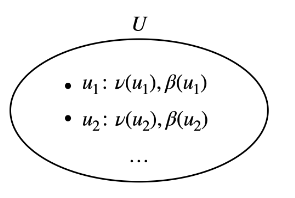
\includegraphics[width=0.5\textwidth]{../assets/discrete-money-distribution.png}
    \caption{Schematic representation of discrete money distribution}
    \label{fig:discrete-md}
\end{figure}

\subsubsection{Using Context}

But the discrete nature of the model does not provide the necessary element for us to add the desired properties to the
payment system. Here we propose a modification that involves the usage of \textit{context ($\gamma$)}:

\begin{figure}[h]
    \centering
    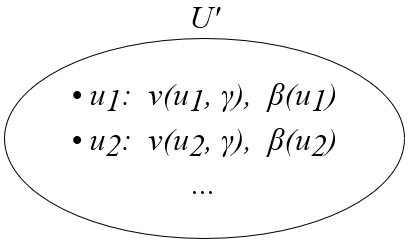
\includegraphics[width=0.5\textwidth]{../assets/money-distribution-with-ctx.png}
    \caption{Schematic representation of money distribution with context}
    \label{fig:md-with-ctx}
\end{figure}

Note that in this model, context can be updated independently while value functions of the same money distribution can
produce different monetary values.

\paragraph{}

Here are some examples how that could work:

\begin{itemize}
\item If time (t) is included the context, then monetary value of each monetary unit can be continuous over time. Time
    is part of the physical reality, hence not changeable by the actors in the payment system.
\item Any subset of monetary units can also have their value functions depending on the same information in
    context. This could enable payment primitives that involve many parties. This set of information in context is
    referred to as \textit{ctx :: SharedContext}, they can be changed over time by the actors in the payment system.
\end{itemize}

For the purpose of this paper, the model of context is: $\gamma = (t :: Timestamp) \oplus (ctx :: SharedContext)$.

\subsubsection{Haskell Definition Of Money Distribution}

\input{MoneyDistribution.lhs.tex}


\subsection{Payment Primitives}
%%%%%%%%%%%%%%%%%%%%%%%%%%%%%%%

Payment primitives are functions that takes a money distribution, shared context, some payment instruction (args) and
timestamp as inputs and incremental updates\footnote{Specifically being monoidal, that is in short a set that has
associative binary operation and an identity element. See \url{https://ncatlab.org/nlab/show/monoid}.} of money
distribution and shared context as outputs:

\begin{minted}[escapeinside=||,mathescape=true]{haskell}
    somePaymentPrimitive :: ( Timestamp t
                            , MoneyDistribution md
                            , SharedContext ctx
                            , PaymentInstruction args
                            , Monoid md, Monoid ctx
                            )
                         => md |$\otimes$| ctx -> args -> t -> md |$\otimes$| ctx
\end{minted}

Loosely speaking, it is considered a primitive, if it can not be broken down into other existing primitives which result
in the same money distribution; additionally primitives should be the only constructs in a payment system that can
update money distribution.

Updates are \textit{monoidal}, so that they can be incremental and their parallel executions can be modeled.

The best known primitive is instant transfer of monetary value between one monetary unit to another. The introduction of
context enables more primitives to be defined, and this will be discussed in later chapters.


\subsection{Payment Execution Environment Models}
%%%%%%%%%%%%%%%%%%%%%%%%%%%%%%%%%%

\input{FinancialContract.lhs.tex}


\subsection{Money Medium Models}
%%%%%%%%%%%%%%%%%%%%%%%%%%%%%%%%

An attempt of creating a unifying theory for money and its distribution was made by Buldas, Saarepera et
al.\cite{buldas2021unifying}

\begin{displayquote}
A useful observation about existing money schemes is that they all have some kind of monetary units that are physical or
digital representations of money. Examples are bills, coins, bank accounts, Bitcoin UTXOs, etc. \cite{buldas2021unifying}
\end{displayquote}

%%%%%%%%%%%%%%%%%%%%%%%%%%%%%
\section{Relevant Approaches}
%%%%%%%%%%%%%%%%%%%%%%%%%%%%%

\subsection{Constraint Programming}
%%%%%%%%%%%%%%%%%%%%%%%%%%%%%%%%%%%

\subsection{Functional Reactive Programming}
%%%%%%%%%%%%%%%%%%%%%%%%%%%%%%%%%%%%%%%%%%%%

\subsection{Denotational Semantics}
%%%%%%%%%%%%%%%%%%%%%%%%%%%%%%%%%%%

%%%%%%%%%%%%%%%%%%%%%%%%%%%%%%%%%%%%%%%%%%%%%%%%%%%%%%%%%%%%%%%%%%%%%%%%%%%%%%%%%%%%%%%%%%%%%%%%%%%%%%%%%%%%%%%%%%%%%%%%
\chapter{General Payment Primitives}
%%%%%%%%%%%%%%%%%%%%%%%%%%%%%%%%%%%%%%%%%%%%%%%%%%%%%%%%%%%%%%%%%%%%%%%%%%%%%%%%%%%%%%%%%%%%%%%%%%%%%%%%%%%%%%%%%%%%%%%%

%%%%%%%%%%%%%%%%%%%%%%%%%%%%%%%%
\section{Denotational Semantics}
%%%%%%%%%%%%%%%%%%%%%%%%%%%%%%%%

Here is the specification of denotational semantics that support both discrete and continous payments.

Here is the list of acronyms used:

\begin{itemize}
    \item \textbf{MD} is \textit{Money Distribution}.
    \item \textbf{MU} is \textit{Monetary Unit}.
    \item \textbf{RTB} is \textit{Real Time Balance}.
\end{itemize}

\subsection{Generalized Payment Model}

\begin{equation}\label{sem_transfer}
    \begin{split}
        [\![MD\ mu\ t\ rtb]\!] = mu \rightarrow t \rightarrow rtb
    \end{split}
\end{equation}

\subsection{Monoidial Payment Model}
%%%%%%%%%%%%%%%%%%%%%%%%%%%%%%%%%%%%

\begin{equation}\label{sem_mzero}
    [\![\emptyset]\!] = \lambda\ mu\ t\ \rightarrow 0
\end{equation}

\begin{equation}\label{sem_mappend}
    [\![mda \oplus\ mdb]\!] = \lambda\ mu\ t\ \rightarrow
    [\![mda]\!]\ mu\ t\ +\ [\![mdb]\!]\ mu\ t
\end{equation}

\subsection{Payment Primitives}
%%%%%%%%%%%%%%%%%%%%%%%%%%%%%%%

\begin{equation}\label{sem_transfer}
    \begin{split}
        [\![&transfer\ from\ to\ amount\ md]\!] = [\![md]\!]\ \oplus \\
        (\lambda\ case&\ mu\ t \\
        &|\ from = mu \rightarrow -amount \\
        &|\ to   = mu \rightarrow amount \\
        &|\ otherwise \rightarrow 0 \\
        )
    \end{split}
\end{equation}

\begin{equation}\label{sem_updateConstantFlow}
    \begin{split}
        [\![&updateConstantFlow\ from\ to\ flowRate\ t'\ md]\!] = [\![md]\!]\ \oplus \\
        (\lambda\ case&\ mu\ t \\
        &|\ from = mu \rightarrow -flowRate * (t - t') \\
        &|\ to   = mu \rightarrow flowRate  * (t - t') \\
        &|\ otherwise \rightarrow 0 \\
        )
    \end{split}
\end{equation}

\begin{equation}
    unit :: sub \rightarrow subs \rightarrow Int
\end{equation}

\begin{equation}
    proportion\ sub\ subs = {{ unit\ sub\ subs } \over { \displaystyle \sum_{x \in subs} unit\ x\ subs }}
\end{equation}

\begin{equation}\label{sem_distributeProportionally}
    \begin{split}
        [\![&distributeProportionally\ pub\ subs\ amount\ md]\!] = [\![md]\!]\ \oplus \\
        (\lambda\ case&\ mu\ t \\
        &|\ pub = mu \rightarrow -amount \\
        &|\ \exists sub \in subs\ { sub = mu } \rightarrow amount * (proportion\ mu\ subs) \\
        &|\ otherwise \rightarrow 0 \\
        )
    \end{split}
\end{equation}

\begin{equation}\label{sem_distributeProportionally}
    \begin{split}
        [\![&updateProportionalDistributionConstantFlow\ pub\ subs\ flowRate\ t'\ md]\!] = [\![md]\!]\ \oplus \\
        (\lambda\ case&\ mu\ t \\
        &|\ pub = mu \rightarrow -flowRate * (t - t') \\
        &|\ \exists sub \in subs\ { sub = mu } \rightarrow flowRate * (t - t') * (proportion\ mu\ subs) \\
        &|\ otherwise \rightarrow 0 \\
        )
    \end{split}
\end{equation}

%%%%%%%%%%%%%%%%%%%%%%%%%%%%%%%%
\section{Restatement in Haskell}
%%%%%%%%%%%%%%%%%%%%%%%%%%%%%%%%

%%%%%%%%%%%%%%%%%%%%%%%%%%%%%%%%%%%%%%%%%%%%%%%%%%%%%%%%%%%%%%%%%%%%%%%%%%%%%%%%%%%%%%%%%%%%%%%%%%%%%%%%%%%%%%%%%%%%%%%%
\chapter{Superfluid Money - A Reference Implementation}
%%%%%%%%%%%%%%%%%%%%%%%%%%%%%%%%%%%%%%%%%%%%%%%%%%%%%%%%%%%%%%%%%%%%%%%%%%%%%%%%%%%%%%%%%%%%%%%%%%%%%%%%%%%%%%%%%%%%%%%%

\section{Real Time Balance}

\section{Sub Systems}

\section{Agreement Sub System}

\section{Type of Agreements}

\subsection{Transferable Balance Agreement}

\subsection{Constant Flow Agreement}

\subsection{Distribution Agreement}

\subsection{Decaying Flow Agreement}

\section{Solvency Sub Systems}

\subsection{Buffer Based Solvency Systems}

\section{Type Of Monetary Units}

%%%%%%%%%%%%%%%%%%%%%%%%%%%%%%%%%%%%%%%%%%%%%%%%%%%%%%%%%%%%%%%%%%%%%%%%%%%%%%%%%%%%%%%%%%%%%%%%%%%%%%%%%%%%%%%%%%%%%%%%
\chapter{Future Investigations}
%%%%%%%%%%%%%%%%%%%%%%%%%%%%%%%%%%%%%%%%%%%%%%%%%%%%%%%%%%%%%%%%%%%%%%%%%%%%%%%%%%%%%%%%%%%%%%%%%%%%%%%%%%%%%%%%%%%%%%%%

\section{Restatement in Agda and Correctness Proof}

\section{Constraint in Consensus}

\section{Payment in General Accounting Domains}

%%%%%%%%%%%%%%%%%%%%%%%%%%%%%%%%%%%%%%%%%%%%%%%%%%%%%%%%%%%%%%%%%%%%%%%%%%%%%%%%%%%%%%%%%%%%%%%%%%%%%%%%%%%%%%%%%%%%%%%%
\newpage
\printbibliography{}
%%%%%%%%%%%%%%%%%%%%%%%%%%%%%%%%%%%%%%%%%%%%%%%%%%%%%%%%%%%%%%%%%%%%%%%%%%%%%%%%%%%%%%%%%%%%%%%%%%%%%%%%%%%%%%%%%%%%%%%%

\end{document}
